%\documentclass[a4paper, 12pt]{report}
\documentclass[12pt,a4paper,openany]{abntex2}

\usepackage[T1]{fontenc}
%\usepackage[latin1]{inputenc}
%\usepackage[verbose,left=30mm,right=20mm,top=30mm,bottom=30mm]{geometry}
%\usepackage{txfonts}
\usepackage[brazil]{babel}
\usepackage{pdfpages}
%\usepackage[authoryear]{natbib}
%\usepackage{appendix}
%\usepackage{setspace}
%\usepackage{url}
%\usepackage{hyperref}
%\usepackage{color}
\usepackage[utf8]{inputenc}
\usepackage{placeins}
\usepackage{float}

\autor{Leonardo Mendonça de Araujo \and \\ Lucas Bagatini do Nascimento \and \\ Mário Muramatsu Júnior}
\titulo{RELATÓRIO FINAL: IDENTIFICADOR DE SINAIS TRIFÁSICOS}
\data{2018} 
\local{Rio Claro, São Paulo}
\preambulo{Monografia apresentada ao curso de Ciências da Computação, como requisito parcial para a obtenção do Título de Bacharel em Ciências da Computação, Instituto de Geociências e Ciências Exatas da Universidade Estadual Paulista}
\orientador{Mario Roberto da Silva}
\tipotrabalho{monografia}

\begin{document}
	
\imprimircapa	
\imprimirfolhaderosto

\clearpage
\cleardoublepage
\cleardoublepage

\pagenumbering{arabic}
\setcounter{page}{3}

\tableofcontents
\clearpage{\pagestyle{empty}\cleardoublepage}

\listoffigures
\clearpage{\pagestyle{empty}\cleardoublepage}
	
\chapter{Introdução}

\section{Sistemas Elétricos Polifásicos}

Naturalmente, sistemas elétricos funcionando em corrente alternada possuem picos e vales de tensão e, consequentemente, picos e vales de potência. A fim de mitigar esta ineficiência intrínseca, pode-se montar um sistema de corrente alternada polifásico, ou seja, um sistema que fornece energia elétrica através de três ou mais condutores energizados.

As figuras ~\ref{fig:sinal-bifasico} e ~\ref{fig:sinal-trifasico} ilustram o comportamente da tensão em sistemas bifásicos e trifásicos, respectivamente. É trivial perceber que sistemas polifásicos são capazes de fornecer tensão e potência de maneira mais constante e sem necessitar de altos picos em cada uma de suas fases.

\begin{figure}[!htp]
	\centering
	\fbox{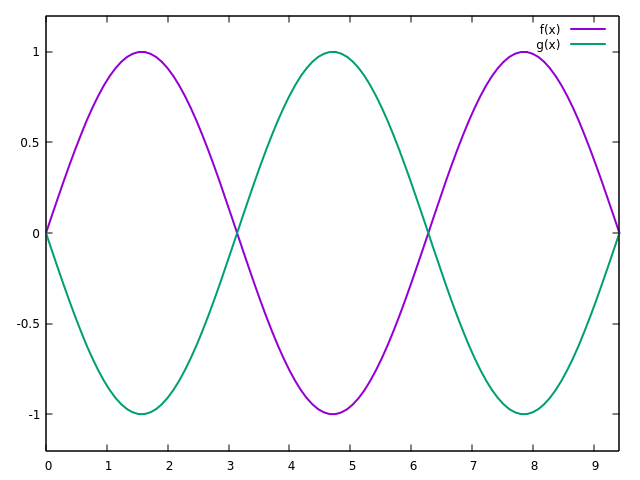
\includegraphics[width=16cm]{./images/Bifasico.png}}
	\caption{Exemplo de sistema Bifásico}
	\label{fig:sinal-bifasico}
\end{figure}

\begin{figure}[!htp]
	\centering
	\fbox{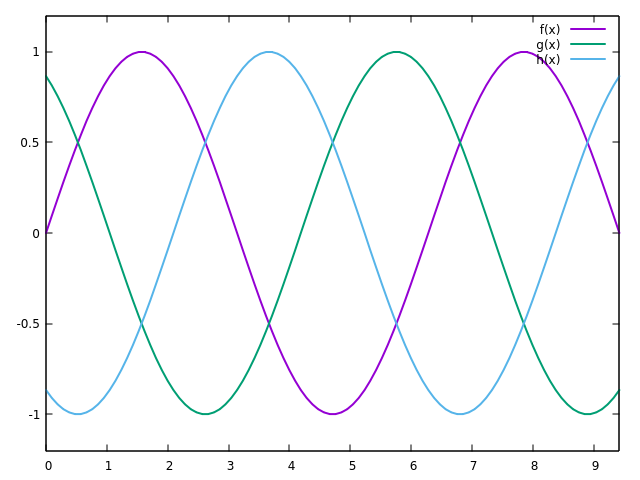
\includegraphics[width=16cm]{./images/Trifasico.png}}
	\caption{Exemplo de sistema Trifásico}
	\label{fig:sinal-trifasico}
\end{figure}

Um sinal trifásico, como da Figura ~\ref{fig:sinal-trifasico}, assim como outras variações de sinais polifásicos, são criados nos geradores; originados dos motores de indução polifásicos desenvolvidos concomitantemente por Galileo Ferraris, Nikola Tesla e Mikhail Dolivo-Dobrovolsky. Um gerador alternador trifásico é composto por um núcleo magnético assim como qualquer outro alternador, e seu estator é composto de bobinas ligadas aos três condutores ao invés de dois, como em um alternador simples. Conforme o rotor gira, este excita os elétrons livres nas bobinas dentro de seu campo magnético, criando corrente alternada. Existe, portanto, uma relação de proporcionalidade direta entre o espaçamento das bobinas e às distâncias das fases em cada um dos condutores.

\begin{figure}[!htp]
	\centering
	\fbox{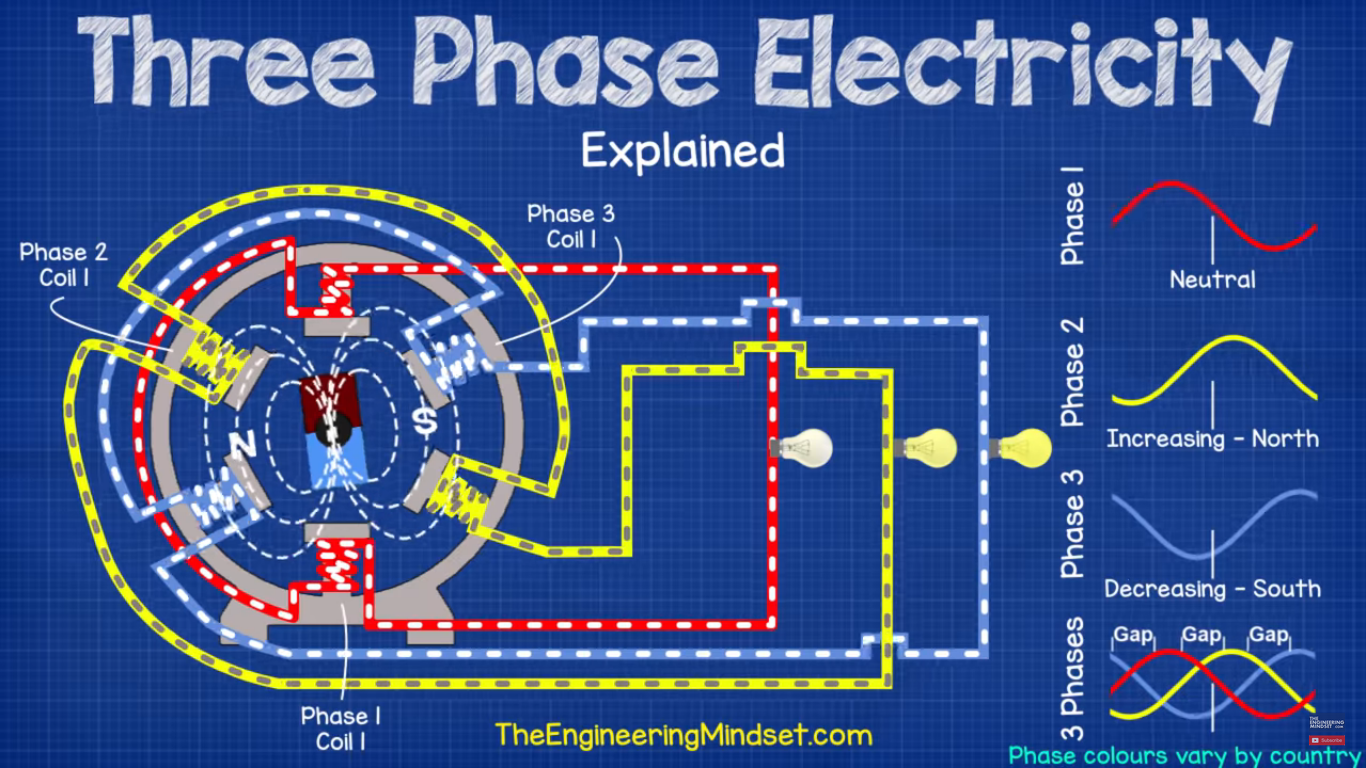
\includegraphics[width=16cm]{./images/EsquemaTrifasico.png}}
	\caption{Esquema de um Alternador Trifásico}
	\label{fig:alternador-trifasico}
\end{figure}


%https://youtu.be/4oRT7PoXSS0?t=345  em 5:45, acessado em 25/10/2018, 20:40

É possível, dada uma instalação trifásica, utilizar somente uma das fases em associação com o neutro para alimentar pequenos aparelhos, como lâmpadas e telas. Portanto, não é necessário ter duas redes elétricas dentro de uma mesma instalação industrial, por exemplo. Geralmente é desta maneira que energia elétrica é distribuída para residências, já que não espera-se que uma família tenha um forno industrial em sua cozinha.

\section{Sistemas Trifásico: Usos e Vantagens}

Como discutido acima, um sistema trifásico de transmissão (que se utiliza de três condutores) de energia possui diversas vantagens sobre sistemas monofásicos (que usam dois condutores). Dentre eles, o mais notório é o ganho em custo-benefício de tal sistema. Pode-se transmitir o triplo da energia com somente 50\% de incremento nos custos. A partir de 3 fases o incremento no custo é grande demais para compensar os benefícios.

Sistemas polifásicos são especialmente úteis e convenientes na construção e operação de motores elétricos, tal qual os motores de indução, por serem capazes de produzirem campos magnéticos rotativos de intensidades mais constantes e confiáveis. É possível alterar a frequência das três fases para alterar a velociade de rotação do motor, por exemplo. Motores de indução que utilizam corrente contínua requerem diversas peças adicionais, como transformadores, que encarecem o mecanismo final. Menores flutuações na potência entregue aos eixos também significa que menor stress será causado ao material, permitindo o uso de materiais mais baratos ou leves, aumentando ainda mais a eficiência e o custo-benefício.https://youtu.be/4oRT7PoXSS0?t=345  em 5:45, acessado em 25/10/2018, 20:40


De maneira análoga à motores de indução, sistemas de distribuição trifásicos são capazes de aproveitar mais da energia gerada por um gerador, como turbinas de uma hidrelétrica.

\section{Projeto: Identificador de Sinais Trifásicos}

Ao longo de grandes instalações elétricas, ao se utilizar modelos trifásicos, deve-se garantir que os diversos dispositivos e conexões estão ligados às fases adequadas. Erros desta natureza podem causar desde ineficiência do maquinário ligado até catastróficos acidentes. A fim de auxiliar na tarefa, propõe-se que seja construído um Identificador de Fase para Sinais Trifásicos.

Sabendo-se que dois condutores fazem parte de um mesmo sistema de transmissão trifásico ou rede de transmissão, o aparato deve ser capaz de fazer a leitura da frequência presente em um e compará-la à frequência do outro, indicando se há ou não defasagem entre ambos. Deve-se construir também um sistema que garanta a confiabilidade da leitura, indicando ao usuário quando o sinal lido anteriormente não é mais confiável. O aparato deve, também, mitigar variações momenâneas causadas pelo início da leitura, tal qual o repetido conecta-desconecta causado pelos imperceptíveis e repetidos choques, natural do contato inicial entre materiais duros, como o metal dos fios e a ponta de prova.

O usuário, após acoplar o aparato a condutor, terá consigo uma amostra da fase obtida através de contadores internos. Ao comparar o conteúdo do aparato com a fase de outro condutor, este indicará se há adianto ou atraso de um terço de um período do segundo em relação ao primeiro. Parte-se do pressuposto que ambos têm frequências iguais, já que são leituras em partes distintas de uma mesma rede ou linha de transmissão.

Pode-se utilizar o aparato para garantir a sincronia entre duas linhas de transmissão distindas, regulando a frequência e fase da corrente alternada que passa por uma delas até que estejam equiparadas.

\chapter{Materiais e Metodologia}

\section{Equipamento: Software e Placa Altera}

A fim de construir o aparato proposto, conceitualizou-se virtualmente o projeto através do software Quartus em sua versão 9.0 com licença universitária.

O software consiste de diversas janelas e abas, principalmente a área de trabalho, para qual e sobre a qual qual podem ser arrastados diversos elementos de hardware como portas lógicas, pinos de entrada e saída, flip-flops, fios e barramentos.

Além da área de trabalho, existe a opção de alterar os componentes do circuito por meio HDL (Linguagem de Descrição de Hardware). Também é possível executar testes funcionais e/ou de tempo para verificar a integridade dos módulos desenvolvidos antes de testá-los na placa física.

A Figura ~\ref{fig:interface-quartus} mostra a interface do usuário do Quartus versão 9.0.

%Figura X (interface-quartus)
\begin{figure}[!htp]
	\centering
	\fbox{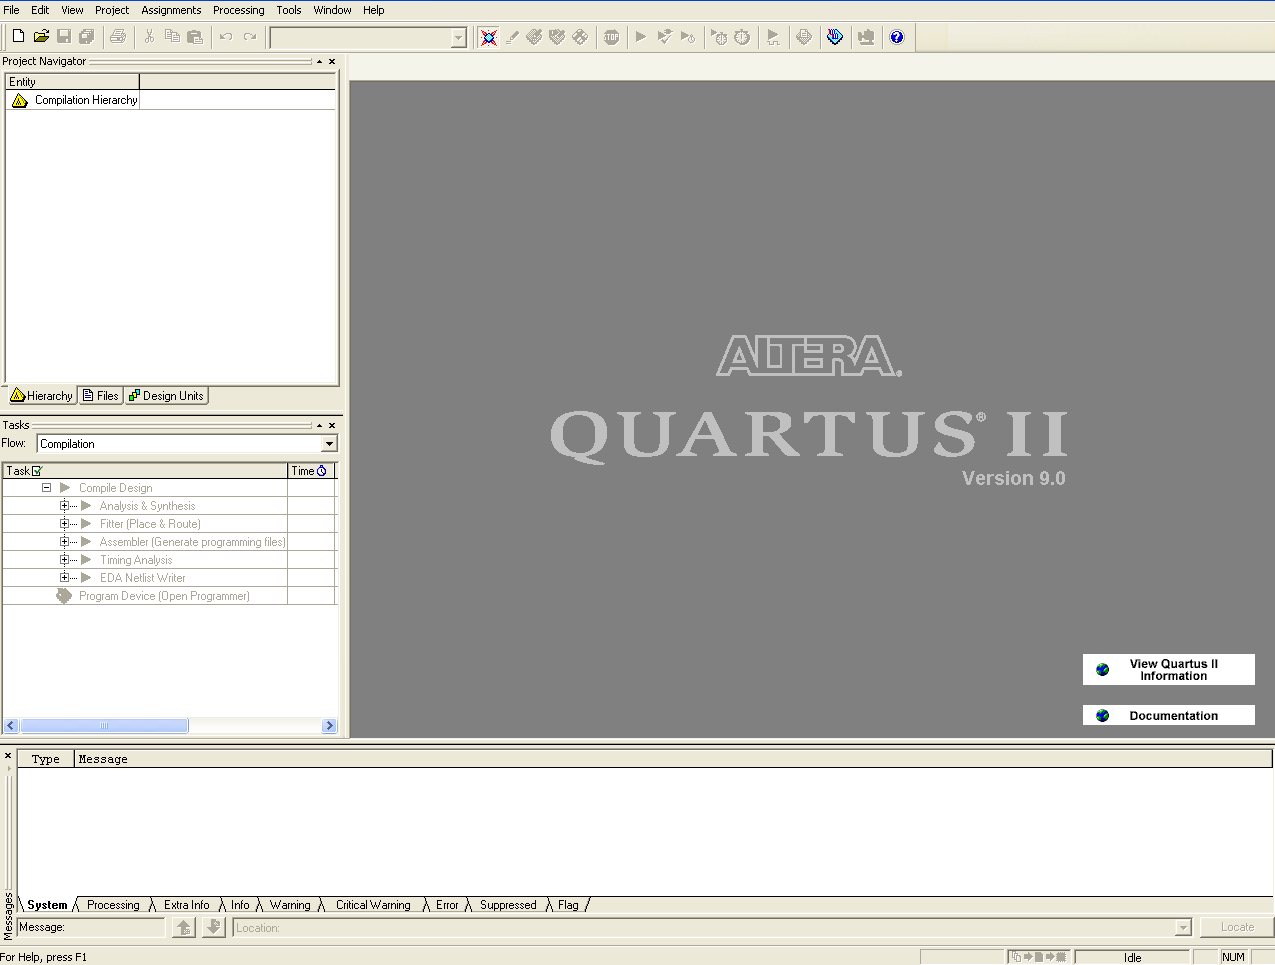
\includegraphics[width=16cm]{images/interface-quartus.png}}
	\caption{Interface do Programa Quartus}
	\label{fig:interface-quartus}
\end{figure}

Em conjunto com o software Quartus versão 9.0, foi usada a placa UP Educational Board para o desenvolvimento e teste de todas as etapas do projeto; representada detalhadamente pela Figura ~\ref{fig:placa-1}.

%Imagem da placa_1
\begin{figure}[!htp]
	\centering
	\fbox{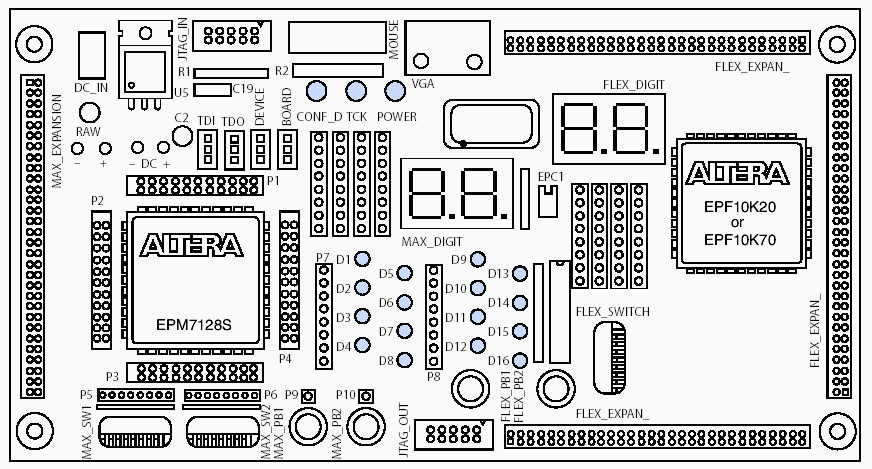
\includegraphics[width=16cm]{images/placa_1.png}}
	\caption{Overview da Placa}
	\label{fig:placa-1}
\end{figure}

Alguns dos elementos da placa utilizados na simulação do funcionamento dos módulos foram os pinos de entrada e saídas de led ( estes últimos para identificar resultados das operações executadas pelo circuito).

%* Explicar necessidade do Antibouncing
\section{Efeito de Bouncing e o Módulo Antibouncing}

Ao trabalhar com aparatos que envolvem peças mecânicas duras e com micro rugosidades, tais como pontas de prova, há a ocorrência de um efeito conhecido como \textit{“bouncing”}. Tal efeito é caracterizado por “idas” e “vindas” ou "conecta-desconecta", causando flutuações imprevisíveis entre leituras (bouncing entre o nível lógico alto e o nível
lógico baixo neste projeto), antes dos sinais tornarem-se efetivamente válidos. O efeito de bouncing tem origem nas forças ação e reação que surgem no contato entre as peças e imperfeições miúdas no material, fazendo com que uma quique na outra por um momento.

As rápidas oscilações provenientes do efeito de bouncing podem
gerar acionamentos indevidos no circuito, já que a interpretação dos sinais é de que o contato (ponta de prova neste projeto) foi acionado repetidas vezes em um curto espaço de tempo, quando, no caso de uma ponta de prova, pretendia-se gerar um único contato.

Com o efeito em mente, viu-se necessário o desenvolvimento de um módulo de Antibouncing integrado ao sistema, capaz lidar com o problema. Utilizando técnicas de desenvolvimento de máquinas sequenciais pode-se fazer com que o sinal de entrada similar ao da Figura ~\ref{fig:sinal-com-bouncing} seja manipulado, gerando uma saída como o apresentado na Figura ~\ref{fig:sinal-sem-bouncing}. Efetivamente, ignora-se as entradas vindas de uma ponta de prova por um período característico de bouncing obtido experimentalmente (função dos materiais e inflenciado pela perícia do operador).

%Imagem A (sinal com bouncing)
\begin{figure}[!htp]
	\centering
	\fbox{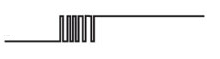
\includegraphics[width=16cm]{images/bounce_on.png}}
	\caption{Sinal com Bouncing}
	\label{fig:sinal-com-bouncing}
\end{figure}

%//Imagem B (sinal sem bouncing)
\begin{figure}[!htp]
	\centering
	\fbox{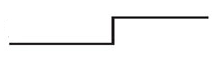
\includegraphics[width=16cm]{images/bounce_off.png}}
	\caption{Sinal sem Bouncing}
	\label{fig:sinal-sem-bouncing}
\end{figure}

* Explicar necessidade do Timeout
\section{Período de Timout e o Módulo de Timeout}

Após implementado o módulo de AntiBouncing, uma nova situação problemática se mostra: o sinal capturado através da ponta de prova (em fase com R, S ou T), com o passar dos segundos degrada-se e se defasa. Depois de um intervalo específico tal defasagem tornar-se-á
tão severa que o sinal já não pode mais ser identificado como R,S ou T claramente, inutilizando a leitura do sinal capturado. Esse período é chamado de \textit{Período de Timeout} do sinal obtido da ponta de prova.

Prova-se necessário, portanto, o desenvolvimento de um módulo adicional integrado ao sistema capaz de cronometrar esse período e identificar quando um sinal capturado através da ponta de prova se torna falível.

Se identificado o sinal não-confiável, um led deve se acender e o aparato pára de funcionar, indicando a necessidade de uma nova leitura do sinal, garantindo novamente um sinal confiável para
ser manipulado pelos outros módulos do circuito.

\chapter{Discussão e Atividades}

\section{Emulador RST}

O primeiro passo para desenvolver o projeto foi criar uma representação do sinal trifásico, para que este sirva de referência para os testes.

A principio, sabemos que os sinais trifásicos possuem defasagem de 120º entre cada onda e assumimos que oscilam a 60Hz (a frequência da rede elétrica AC brasileira). Sendo assim, é necessário criar uma máquina sequencial que seja capaz de gerar tal sinal.

\begin{figure}[!htp]
	\centering
	\caption{Sinais RST}
	\fbox{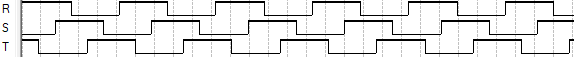
\includegraphics[width=16cm]{images/sinalRST}}
	\label{fig:sinais-rst}
\end{figure}

O primeiro passo foi elaborar um diagrama de sequência que satisfaça as condições para a geração dos sinais.

\begin{figure}[!htp]
	\centering
	\caption{Diagrama de Estado Emulador RST}
	\fbox{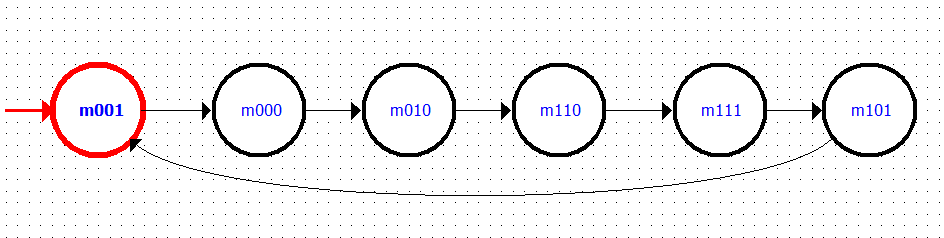
\includegraphics[width=16cm]{images/disgrama-de-estado-EmuladorRST}}
	\label{fig:disgrama-de-estado-EmuladorRST}
\end{figure}

Utilizou-se três bits para referenciar os estados. Note que de um estado para outro apenas um bit é alterado. Foi feita esta escolha pelo fato de que a implementação do circuito seria simplificada. Montou-se a tabela de próximos estados e de excitação dos flip-flops (Figura ~\ref{fig:tabela-RST}).

\begin{figure}[!htp]
	\centering
	\caption{Tabela de estados e excitação dos Flip-flops Emulador RST}
	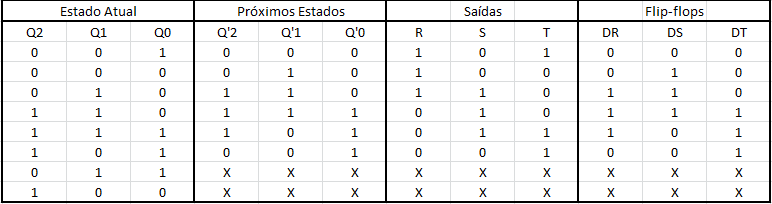
\includegraphics[width=16cm]{images/tabela-RST}
	\label{fig:tabela-RST}
\end{figure}

Utilizando-se do método de Karnaugh para fazer a simplificações e encontrar as expressões de cada saída do circuito, obeve-se o seguinte:

$$DR = Q1$$
$$DS = \overline{Q0}$$
$$DT = Q2$$

As saídas serão:

$$R = \overline{Q2}$$
$$S = Q1$$
$$T = Q0$$

A partir disto, construiu-se o circuito do emulador RST, representado pela Figura \ref{fig:circuito-RST}.

\begin{figure}[!htp]
	\centering
	\caption{Circuito do Emulador RST}
	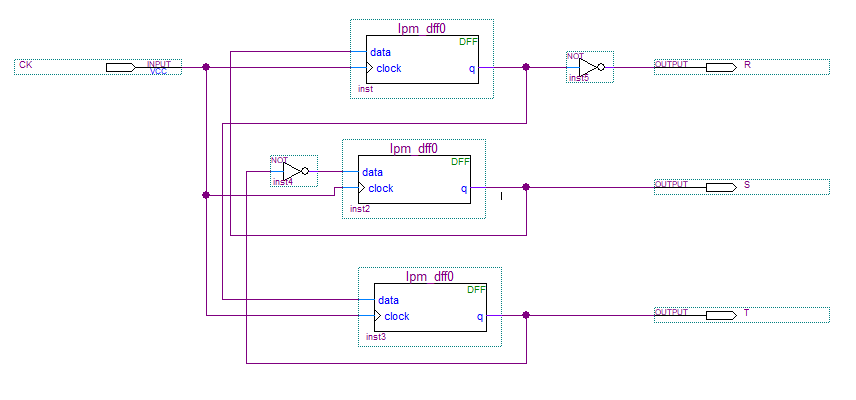
\includegraphics[width=16cm]{images/circuito-RST}
	\label{fig:circuito-RST}
\end{figure}

Tal circuito gera sinais periódicos defasados em 120º. Restava então regular a frequência para 60Hz. Contudo, a placa utilizada possui clock de 25.175MHz; fazendo-se necessário reduzir o clock de entrada do circuito. 

A fim de executar a redução, foi utilizada a saída Carry-out de um contador de módulo 34965 como o clock do circuito RST, garantindo que o clock original seja dividido pelo módulo do contador. O valor obtido foi dividido por 12 posteriormente: dividido por 2 através de um flip-flop tipo T e depois por 6 ao passar pelo emulador RST (por possuir 6 estados).

A Figura \ref{fig:circuito-RST-complete} representa o circuito que gera os sinais corretamente.

\begin{figure}[!htp]
	\centering
	\caption{Circuito do Emulador RST com saídas a 60Hz}
	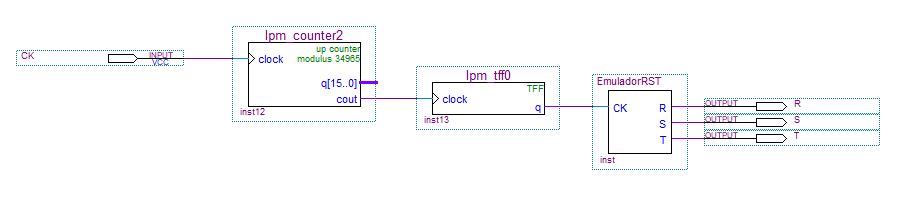
\includegraphics[width=16cm]{images/circuito-RST-complete}
	\label{fig:circuito-RST-complete}
\end{figure}

\section{Aferidor de Período}

Construído o módulo gerador de sinais RST, faz-se necessário ser capaz de receber um sinal de entrada e interpreta-lo para que seja possível dizer com qual das três fases este está em sincronia. 

A  Figura \ref{fig:diagrama-medidor-de-frequencia} descreve o circuito capaz de executar a tarefa.

\begin{figure}[!htp]
	\centering
	\caption{Diagrama esquemático do medidor de período da fase de referência}
	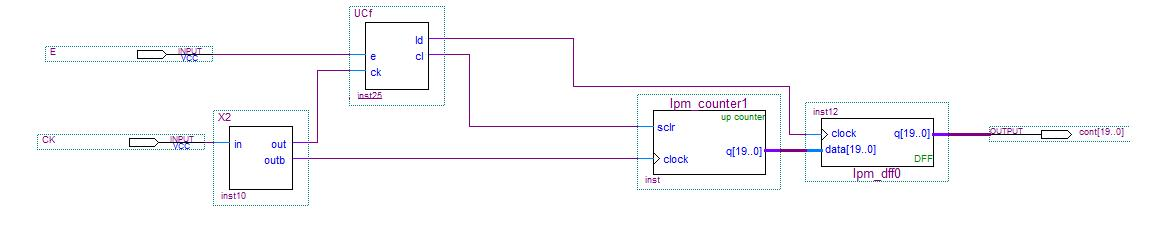
\includegraphics[width=16cm]{images/diagrama-medidor-de-frequencia}
	\label{fig:diagrama-medidor-de-frequencia}
\end{figure}

Sabe-se que o período é toda a extensão desde sua primeira
borda de subida até a sua próxima borda de subida, então, para identifica-lo, utilizou-se um contador que conta o número de ciclos dentro de um período e então armazena-o em um registrador.

Ao inicio de cada período o contador é zerado através do sinal Cl da unidade de controle UCf. A Unidade de Controle será detalhada mais adiante. Entre um clock e outro, na borda de subida, através do sinal Ld, o ultimo valor contado é transferido para o registrador. Para que ambos os comandos sejam executados em ordem correta foi criado a unidade X2.

\begin{figure}[!htp]
	\centering
	\caption{Unidade X2}
	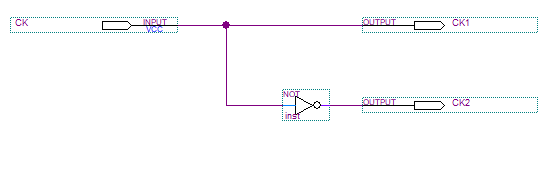
\includegraphics[width=16cm]{images/unidade-x2}
	\label{fig:unidade-x2}
\end{figure}

A única função da unidade da Figura \ref{fig:unidade-x2} é, a partir de uma entrada (no caso o clock), gerar duas saídas: uma idêntica ao sinal de entrada e a outra com o sinal negado.

Note que o clock do contador provém do sinal CK2 de X2, ou seja, tal contador trabalha na borda de descida do clock original. Devido a isto, os comandos Cl e Ld podem ser executados no mesmo clock, uma vez que, assim que forem gerados sinais altos de Cl e Ld, na borda de subida do clock, o valor contado pelo contador é salvo no registrador e no borda de descida deste mesmo clock, é feito o clear do contador.

\section{Correção de Erro aleatório}

Ao utilizar a unidade X2 para sincronizar os comandos, insere-se um erro aleatório à contagem. Há dois casos extremos:

\begin{itemize}	
	\item O sinal de entrada é inserido exatamente antes da borda de subida do clock, fazendo com que a zeragem do contador possua um atraso de 0,5 clock, ou seja, um erro de -0,5 clock, porém note que no valor registrado é desconsiderado 0,5 clock, com isto é gerado mais um erro de -0,5 clock, mostrado na Figura \ref{fig:erro-leitura1};
\end{itemize}


\begin{itemize}	
	\item O sinal de entrada é inserido exatamente depois da borda de subida do clock e o contador é zerado com um atraso de 1,5 clocks, ou seja, com um erro de -1,5 clocks. Além disso, o valor é registrado com 1 clock a mais, gerando um erro de +0,5 clock na leitura, representado pela Figura \ref{fig:erro-leitura2}.
\end{itemize}

\begin{figure}[!htp]
	\centering
	\caption{Entrada exatamente antes da borda de subida}
	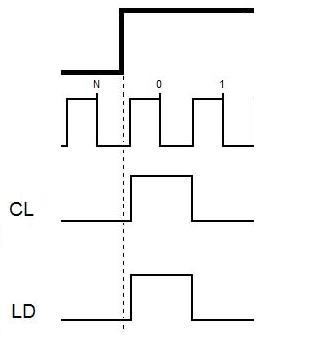
\includegraphics[width=7cm,height=7cm]{images/erro-leitura1}
	\label{fig:erro-leitura1}
\end{figure}

\begin{figure}[!htp]
	\centering
	\caption{Entrada exatamente depois da borda de subida}
	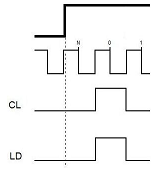
\includegraphics[width=7cm,height=7cm]{images/erro-leitura2}
	\label{fig:erro-leitura2}
\end{figure}

Analisando todas as combinações de erros possíveis nos dois casos extremos e utilizando a operação de convolução para estimar a probabilidade conjunta do dois eventos (carga e zeragem), conclui-se que há a inserção de um erro aleatório variando com distribuição de probabilidade com centro em -1 e bordas em -2 e 0 tal qual mostrado na Figura \ref{fig:distribuicao-de-probabilidade-do-erro}.

\begin{figure}[!htp]
	\centering
	\caption{Distribuição de probabilidade do erro}
	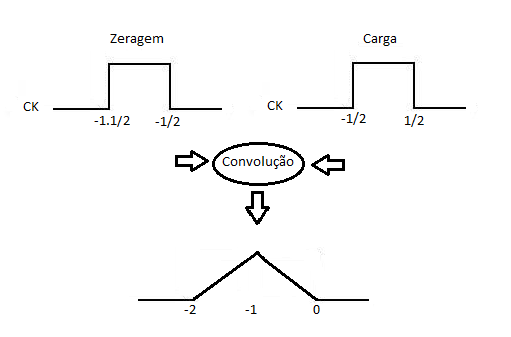
\includegraphics[width=14cm,height=10cm]{images/distribuicao-de-probabilidade-do-erro}
	\label{fig:distribuicao-de-probabilidade-do-erro}
\end{figure}

Note que, pelo fato da distribuição ter centro em -1, o erro mais comum é o de -1 clock, ou seja, a cada leitura será perdido um clock da fase de entrada, tornando as leituras imprecisas. 

O ideal nesta situação seria se centro da curva de distribuição de probabilidade estivesse centrada em 0, tornando a variação mais provável a de 0 clocks, garantindo a integridade da leitura.

No primeiro circuito, o contador possuía uma entrada sclr (Synchronous Clear), este comando permite zerar todos os bits do contador; porém, para corrigir tal problema alterou-se esta entrada para um sset (Synchronous set). Este comando insere um valor preestabelecido, no caso, 1.

Desta forma garante-se a inserção de um erro de +1 clock na leitura, uma vez que o primeiro clock não será contado, e sim inserido. Isso faz com que a distribuição de probabilidade atinja o comportamento ideal, ou seja, somando 1 ao erro aleatório o centro da curva ficará em 0, representado pela Figura \ref{fig:distribuicao-de-probabilidade-do-erro1}.

\begin{figure}[!htp]
	\centering
	\caption{Distribuição de probabilidade do erro com centro em 0}
	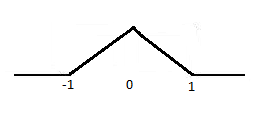
\includegraphics[width=8cm,height=5cm]{images/distribuicao-de-probabilidade-do-erro1}
	\label{fig:distribuicao-de-probabilidade-do-erro1}
\end{figure}

Note que esta solução não previne que hajam erros; apenas diminui a probabilidade de que ocorram. Para que seja possível garantir que o sinal lido é confiável, foi criado um outro circuito que visa promover isto, o qual será apresentado e descrito mais a frente.

\section{Gerador}

Até este estágio o circuito era  capaz de aferir o período de um sinal de entrada. Contudo, o exforço será perdido se a ponta de prova for desconectada do condutor fornecendo o sinal. Pretendia-se então, criar um circuito capaz de gerar um sinal em sincronia com o sinal de referência recebido. 

Primeiramente construiu-se um diagrama de estados para uma UC (Unidade de Controle) capaz de gerenciar os componentes do circuito com o objetivo de fazer a cópia do sinal recebido, representada pela Figura \ref{fig:diagrama-de-estado1}.

\begin{figure}[!htp]
	\centering
	\caption{Diagrama de estados da nova UC}
	\fbox{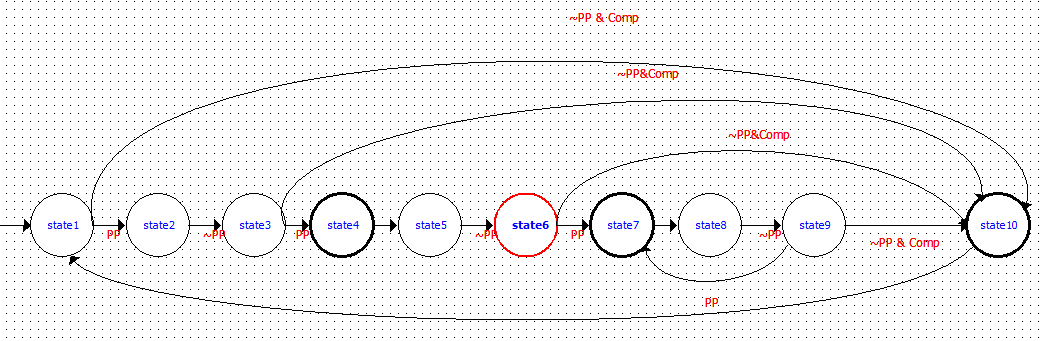
\includegraphics[width=16cm]{images/diagrama-de-estado1}}
	\label{fig:diagrama-de-estado1}
\end{figure}

Ao conectar um sinal de entrada ao circuito, este estará no estado 1 do diagrama, e então irá para o estado 2 quando PP (sinal de entrada) estiver em 1. Para passar para o estado 3 é necessário que PP esteja em 0. Este processo tem como objetivo descartar o primeiro período, pois há possibilidade de este estar fragmentado, gerando leituras errôneas e inúteis.

Chegando ao estado 4, o sinal Cl permanecerá em nível alto, limpado assim o contador. Em seguida passa-se para o estado 5 que, junto com o estado 6, esperarão que outro período se transcorra, atingindo finalmente o estado 7, em que são gerados sinais Cl e Ld. Garantida a primeira aferição do período, a máquina evolui sucessiva e repetidamente pelos estados 8, 9 e de volta para o 7, nos quais são providos os sinais Cl e Ld, permitindo a realização de novas e corretas medições, sobrescrevendo umas às outras, até que o sinal de entrada seja retirado e o sinal Comp esteja em 1.

O sinal Comp permanecerá em 1 sempre que o contador atingir o valor lido nos estado 4, 5 e 6, ou seja, quando completar um período da fase de entrada.

No estado 10, é gerado um sinal Cl para manter o sincronismo com a fase lida e então a maquina retorna para o estado 1. A partir deste ponto o a maquina fica repetidamente indo do estado 1 para o 10 e  depois para 1 novamente, esta transição irá ocorrer sempre que o sinal de entrada estiver em 0 e o Comp estiver em alto, ou seja, sempre ao fim de um período.

A partir deste diagrama de estado pode-se construir o circuito da Figura \ref{fig:gerador}. Note que reaproveitou-se parte do circuito: o contador e o registrador. O comparador abaixo (inst 11) faz a comparação entre o sinal corrente e o valor de frequência armazenado, gerando assim o sinal Comp que é utilizado pela UC. Tal sinal, possui um ciclo ativo muito pequeno, que impede a visualização deste em um osciloscópio, a fim de gerar um sinal capaz de ser visualizado foi inserido o comparador na parte superior (inst 10), que irá comparar a contagem em curso com a metade da contagem registrada que será obtido do registrador de deslocamento ao lado (inst 5), fazendo com que o sinal "copia" de saída possua ciclo ativo de 50\% síncrono com o sinal de entrada.

Outra mudança necessária foi a troca do registrador (inst9) para um que começasse com o valor máximo possível (isto é, todos os bits em 1). Isto se deve pois, como o lpm\_counter1 (inst 8) começa sempre em 1, e se o comparador começar em 0, o sinal Comp não seria ativado corretamente.

\begin{figure}[!htp]
	\centering
	\caption{Diagrama de estados da nova UC}
	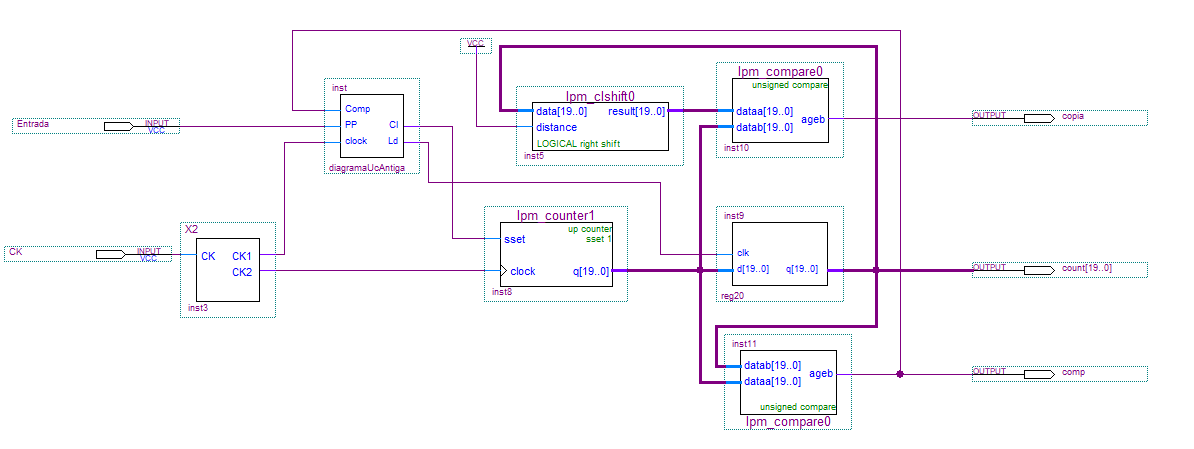
\includegraphics[width=16cm,height=7cm]{images/gerador}
	\label{fig:gerador}
\end{figure}

\section{Comparador de Fase}

Após inserir um sinal de entrada, o circuito é capaz de gerar uma cópia desta fase, porém, é impossível descobrir qual fase foi inserida (R, S ou T). Implementou-se três botões - Rin, Sin e Tin - que devem ser pressionados pelo usuário para indicar qual fase foi aferida inicialmente.

Ao pressionar um dos botões de entrada, a saída LedOutput deve ser equivalente ao botão pressionado, isso acontece até que se tire o dedo do botão. Assim quando chegar um novo sinal de Clear, não existirá mais sinal desses botão; a saída, contudo, deve permanecer a mesma. Isso porque a lógica do componente saidaLed é realimentada com os valores de Rout, Sout e Tout. Apenas ocorrerá alteração na saída ao colocar um novo sinal na ponta de prova.

\subsection{Máquina sequencial CompFase}

Neste ponto, a máquina está pronta para executar a leitura de uma nova fase para fazer a comparação. A máquina sequencial da Figura \ref{fig:comp-fase} sinaliza se o novo sinal de entrada está em sincronia em relação à fase de referencia, se é a fase anterior (na sequencia RST) ou a fase posterior, para isto utiliza a seguinte lógica:
\begin{itemize}
	\item estados começando em 00, indicam que a fase inserida é igual a fase de referencia;
	\item estados começando em 01, indicam que a fase inserida é a posterior à fase de referencia;
	\item estados começando em 10, indicam que a fase inserida é a anterior à fase de referencia.
\end{itemize}

Perceba que o ultimo bit serve para diferenciar os estados cujos valores de saídas são iguais.

\begin{figure}[!htp]
	\centering
	\caption{Diagrama de estados da comparadora de fases}
	\fbox{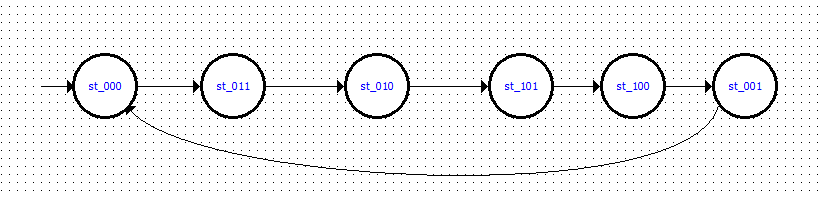
\includegraphics[width=16cm,]{images/comp-fase}}
	\label{fig:comp-fase}
\end{figure}

\subsection{Circuito CompFase}

A partir da máquina sequencial apresentada, pode-se construir o circuito da Figura \ref{fig:circuito-compfase}.

\begin{figure}[!htp]
	\centering
	\caption{Circuito CompFase}
	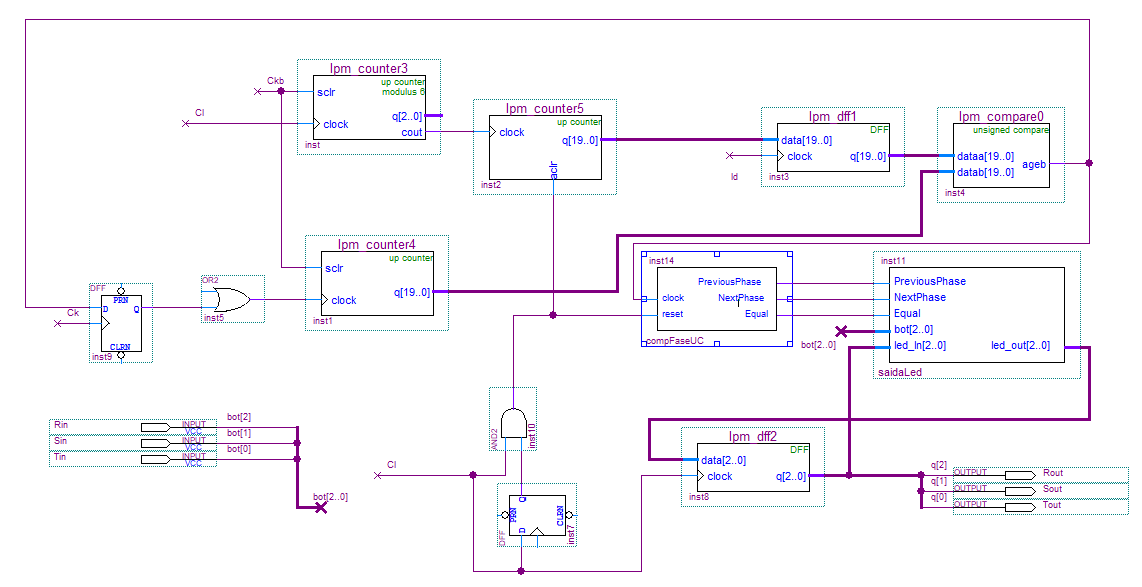
\includegraphics[width=16cm]{images/circuito-compfase}	\label{fig:circuito-compfase}
\end{figure}

Utilizar o método de comparação de fases requer uma frequência de seis vezes a frequência da fase de referência. Assim, o contador Ipm\_counter3 (inst) gera esta frequência dividindo o clock por seis, sendo então utilizado para realizar uma contagem entre as bordas de subida da fase de referência pelo contador Ipm\_counter5 (inst2), resultando em uma contagem truncada em $\frac{1}{6}$ do período da fase de referência, sendo armazenada em um registrador Ipm\_dff1 (inst3) pelo pulso Ld.

Como o contador Ipm\_counter5 (inst2) recebe um clock com $\frac{1}{6}$ da
frequência original do circuito, é utilizado um Clear assíncrono que ocorre na borda de descida anterior ao pulso Cl, com metade de sua duração, proveniente da porta "E" AND2 (inst10) entre o pulso Cl e o flip-flop tipo D DFF (inst9), que também realiza o Clear na máquina comparadora de fases.

O comparador Ipm\_compare (inst4) provém então o clock necessário para a
máquina comparadora de fases, e realiza também o Clear do contador Ipm\_counter4 (inst1), através da comparação entre a contagem truncada em $\frac{1}{6}$ do período da fase de referência e a do próprio contador, após o atraso de meio período de clock, obtido com o flip-flop tipo D DFF (inst9), pois sua saída também ocorre em uma borda de descida. Como uma divisão por seis pode envolver resto, o contador Ipm\_counter4 (inst1) também recebe outro sinal de Clear através da porta "OU" OR2 (inst5) produzido a cada período da fase de referência, evitando-se o acúmulo de erros.

\section{Timeout}

Na seção 3.3, na qual o problema de erro aleatório na leitura da fase de referência corrigiu-se o problema do erro aleatório, foi dito que aquilo era o suficiente para acabar com os erros de leitura, uma vez que, os erros variam de acordo com uma distribuição de probabilidade continua com centro em 0, isto é, pode variar de -1 a +1 clock de erro.

Este valor pode parecer pequeno, mas este erro se repete a cada novo período enquanto se espera a conexão da nova fase de referência à ponta de prova. O sinal gerado internamente se defasa em relação à fase de referência para mais ou para menos.

Se o acumulo deste erro se tornar suficientemente grande, a comparação perde sua validade. Se a fase R for inserdia como referência, por exemplo, após a cópia se defasar em $\frac{1}{6}$ para menos em relação a fase de referencia e inserindo novamente uma fase R para fazer a comparação, tal situação se confunde com o caso em que é inserido a fase S para fazer a comparação e a cópia se defasou em $\frac{1}{6}$ para mais.

Para corrigir isto criou-se o circuito Timeout, que nada mais é do que um temporizador. Este circuito ira executar uma contagem decrescente, até que a fase de referencia esteja defasada (situação limite é quando esta atinge $\frac{1}{6}$ de erro). Ao atingir o valor 0, a máquina será travada, indicando que o sinal copiado não é mais confiável, necessitando de uma nova leitura para a fase de referencia.

O tempo deste Timeout pode ser estimado, sendo sua fórmula do tipo: $$Timeout = \frac{Clock}{\left(\left. 6 \right. . \left. \left(frequencia\right)^2\right.\right)}$$

Sendo o clock da placa igual a $25175$MHz e a frequência da rede entre $60$Hz a $70$Hz, temos o tempo aproximadamente de $856s$, equivalente a 14 minutos e 16 segundos.

\subsection{Circuito contador}

Para fazer a contagem, construiu-se o circuito da Figura \ref{fig:timeout}.

O contador lpm\_counter5 (inst8) dividirá o clock de $25175$MHz por dois, gerando um sinal de $2$Hz que será divido novamente por 2 pelo flip-flop tipo T gerando um sinal de $1$Hz. Tal sinal é então dividido pelo contador de módulo 60 (inst3) produzindo um pulso a cada minuto. Os contadores à direita irão receber estes sinal, sendo que os dois superiores executam a contagem em segundos e os inferiores a contagem em minutos, o cout dos contadores de unidades servem para acionar os contadores de dezenas.

O valor inicial calculado acima é inserido através dos pinos aset (Asynchronous Set) dos contadores.

\begin{figure}[!htp]
	\centering
	\caption{Circuito de contagem do timeout}
	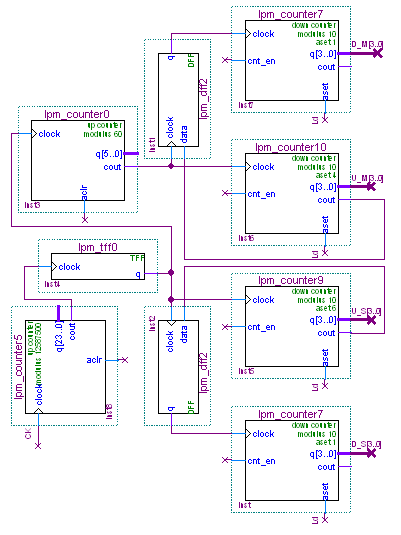
\includegraphics[height=13cm]{images/timeout}
	\label{fig:timeout}
\end{figure}

Quando tais contadores de tempo em minutos alcança 00 é produzido o sinal que deverá travar a máquina toda até que nova fase seja colocada na ponta de prova e esta seja identificada pelo pressionar de um dos botões.

\subsection{Circuito apresentador do Timeout}

Ao atingir o valor de 2 minutos, o contador de segundo deverá estar com tempo restante de 20 segundos, após passar este tempo, a contagem passará a mostrar apenas o valor em segundos, sendo o que este começará em 99 segundos. A combinação entre o valor 2 dos minutos com o 9 dos segundos gera o sinal MIN\_SEC que irá alterar a contagem apenas para segundos. O circuito que faz tão função é representado pela Figura \ref{fig:display-timeout}

\begin{figure}[!htp]
	\centering
	\caption{Circuito do display do Timeout}
	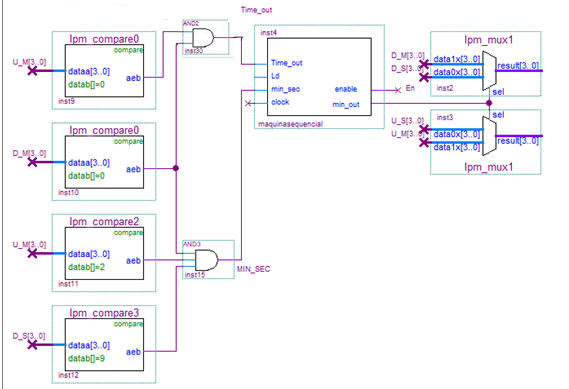
\includegraphics[width=16cm]{images/display-timeout}	\label{fig:display-timeout}
\end{figure}

O bloco lógico Time\_out é representado pelo seguinte diagrama de estado, Figura \ref{fig:diagrama-de-estado-display-timeout}. O circuito irá para o estado 3, onde a contagem de minutos esta ativa, nos estados 1 e 2, a contagem de minutos é desativada. Quando a máquina está nos estados 2 e 3, os pinos enable dos contadores estarão ativos, liberando os contadores para continuarem a contar, porém, no estado 1 estes enables são desativados, travando a contagem.

\begin{figure}[!htp]
	\centering
	\caption{Diagrama de estado do diplay do Timeout}
	\fbox{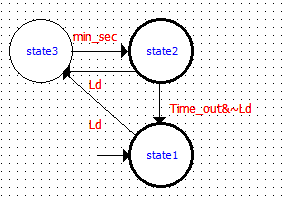
\includegraphics{images/diagrama-de-estado-display-timeout}}
	\label{fig:diagrama-de-estado-display-timeout}
\end{figure}

A transição do estado 3 para o 2 ocorre quando o sinal MIN\_SEC estiver em 1, ou seja, quando a contagem atinge 99 segundos. No estado 2, caso a ponta de prova seja conectada antes do termino do tempo de timeout, a máquina voltará para o estado 3, do contrario ele irá para o estado 1, onde irá ficar travada até que aja uma nova leitura na ponta de prova.

\section{Anti bouncing}

%Ao conectar a ponta de prova ao sinal de referencia ocorre um fenômeno chamado de bouncing, que consistem em oscilações aleatórias geradas pelo contato mecânico entre o fio e a ponta de prova. Isto ocorre devido à condição física dos conectores, uma vez que estes possuem uma superfície rugosa causando uma instabilidade inicial, que provocam pequenas oscilações. Este fenômeno é representado pela Figura \ref{fig:bounceTimingDiagram}

\begin{figure}[!htp]
	\centering
	\caption{Fenômeno Anti bouncing}
	\fbox{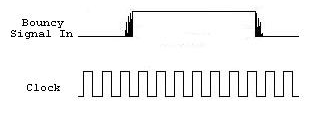
\includegraphics[width=10cm,height=4cm]{images/bounceTimingDiagram}}
	\label{fig:bounceTimingDiagram}
\end{figure}

As oscilações geradas pelo efeito de bouncing (Fig ~\ref{fig:bounceTimingDiagram}) são capazes de influenciar os resultados, fazendo com que a máquina sequencial transite pelos estados sem ter um sinal confiável.

Para corrigir este problema, foi proposta a seguinte máquina sequencial (Figura \ref{fig:antibouncing-diagrama}) que servirá como Unidade de controle do gerador da cópia. Basicamente ela irá travar a leitura até que se passe um tempo necessário para as entradas se estabilizarem, chamado Tempo Característico de Bouncing.

\begin{figure}[!htp]
	\centering
	\caption{Diagrama de estado da Unidade Anti bouncing}
	\fbox{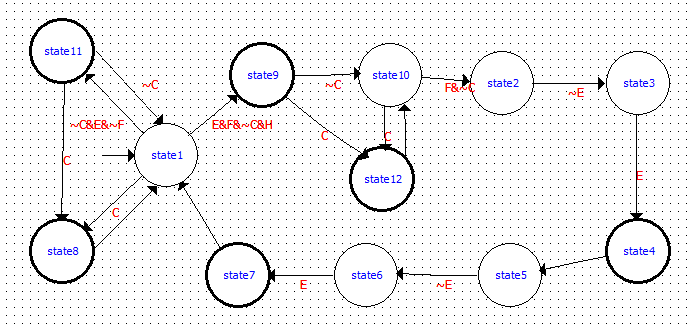
\includegraphics{images/antibouncing-diagrama}}
	\label{fig:antibouncing-diagrama}
\end{figure}

Ao iniciar a máquina, ela permanecerá no estado 1 até que uma ponta de prova seja conectada ao dispositivo e o tempo característico de bouncing ja tenha passado e o sinal H, que é recebido através do pressionar de um dos botões que indicam qual é a fase inserida, esteja em 1. Se estas condições forem cumpridas então a máquina evoluirá para o estado 9, onde produzirá um sinal Rf (Reset Flag), por um clock, e irá para o estado 12 caso o sinal Comp esteja em 1, do contrário irá para 10. O caso em que Comp estiver em 1 significa que houve um transcurso de mais um período registrado, para isto, é necessário então que o sinal Cl esteja em 1, Cl é colocado em nível alto, por um clock, no estado 12 e em seguida ele irá para o estado 10.

A máquina ficará no ciclo entre o estado 10 e 12 até que o sinal F esteja em 1, ou seja, até passar o tempo característico de bouncing. Os estados 2 e 3 irão permitir a detecção da próxima borda de subida da fase. No estado 4, é gerado um sinal Cl, que irá zerar o contador de período, no estado 5 e 6 seja possível fazer a contagem do período corretamente e então salvando-o no estado 7 com um sinal Ld e outro Cl, para finalmente retornar ao estado 1.

Neste ponto, sempre que o sinal Comp estiver em 1 a máquina irá para o estado 8, em que será gerado um sinal Cl para mantar o sincronismos com a fase de referencia. Caso a ponta de prova ainda esteja conectada e em nível alto, a máquina irá para o estado 11, para gerar um sinal Rf para impedir que F seja ativada, e logo em seguida irá voltar para o estado 1 ou primeiro irá para o estado 8, pela necessidade de um clear e em seguida retornará ao 1.

A partir deste diagrama foi construído o circuito da Figura \ref{fig:antibouncing-uc}.

\begin{figure}[!htp]
	\centering
	\caption{Circuito da Unidade de controle com Anti bouncing}
	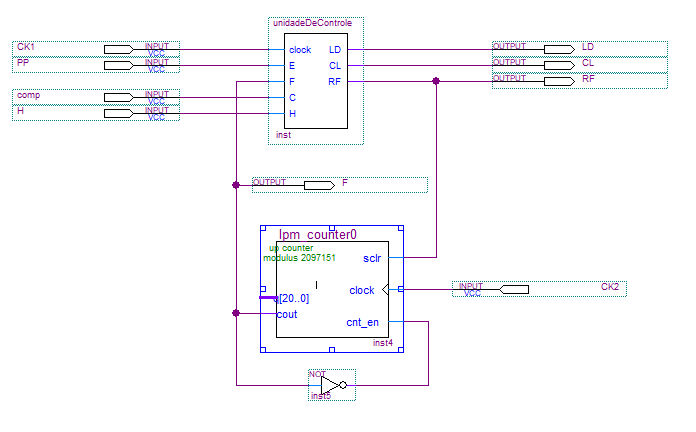
\includegraphics[width=16cm]{images/antibouncing-uc}	\label{fig:antibouncing-uc}
\end{figure}

O sinal Rf que é gerado para não permitir que a entrada F esteja em 1 nada mais é do que um sclr (Synchronous clear) do lpm\_counter (inst14). Este contador irá marcar o tempo característico de bouncing, ao final desta contagem, o sinal cout (Carry out) será expelido, indicando que o contador atingiu o seu limite, ou seja, passou-se o tempo necessário. Note que esta saída influencia o próprio contador, uma vez que o sinal cout é inserido na entrada cnt\_en (Counter Enable). Ao inseri-la, o contador será desativado, até que seja dado um clear.

\chapter{Resultados e Discussão}

\subsection{Teste - Circuito RST}

O primeiro circuito implementado foi o gerador de sinais RST, pois este serviria para fazer todos os testes seguintes. Para que fosse possível visualizar a variação das ondas geradas pelo circuito, foi necessário diminuir o valor do contador de lpm\_counter2 (inst12) da Figura \ref{fig:circuito-RST-complete}, pois este estaria variando a 60Hz, algo que dificultaria a visualização. Alterando o valor para 10 chegamos aos resultados da Figura \ref{fig:teste-rst}.

\begin{figure}[!htp]
	\centering
	\caption{Simulação funcional com o emulador de sinais RST}
	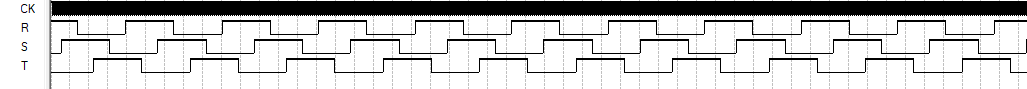
\includegraphics[width=16cm]{images/teste-rst}	\label{fig:teste-rst}
\end{figure}

Assim como o esperado o circuito é capaz de gerar três ondas defasadas em 120º, podendo concluir que tal circuito apresenta uma representação próxima ou até mesmo fiel à situação real.

Este circuito foi testado na placa utilizando os displays de 7 seguimentos presentes nela. Cada sinal RST era representado por um seguimento, quando o sinal de uma das fases ficasse em nível alto, o seu respectivo seguimento era aceso. 

\subsection{Teste - Gerador e Anti bouncing}



Para conseguir testar esta parte foi necessário assumir quer o sinal H sempre estaria em 1; isto porque a parte da implementação dos botões que indicariam qual é a fase de entrada não havia sido implementada até então. O sinal de entrada utilizado foi gerado pelo emulador RST e para simular o fenômeno de bouncing utilizamos um multiplexador que simularia uma instabilidade na entrada.
2777 ns
O teste foi feito com o clock em 2777ns no circuito da Figura \ref{fig:teste-antibouncing}.

\begin{figure}[!htp]
	\centering
	\caption{Circuito de testes do Gerador e Anti bouncing}
	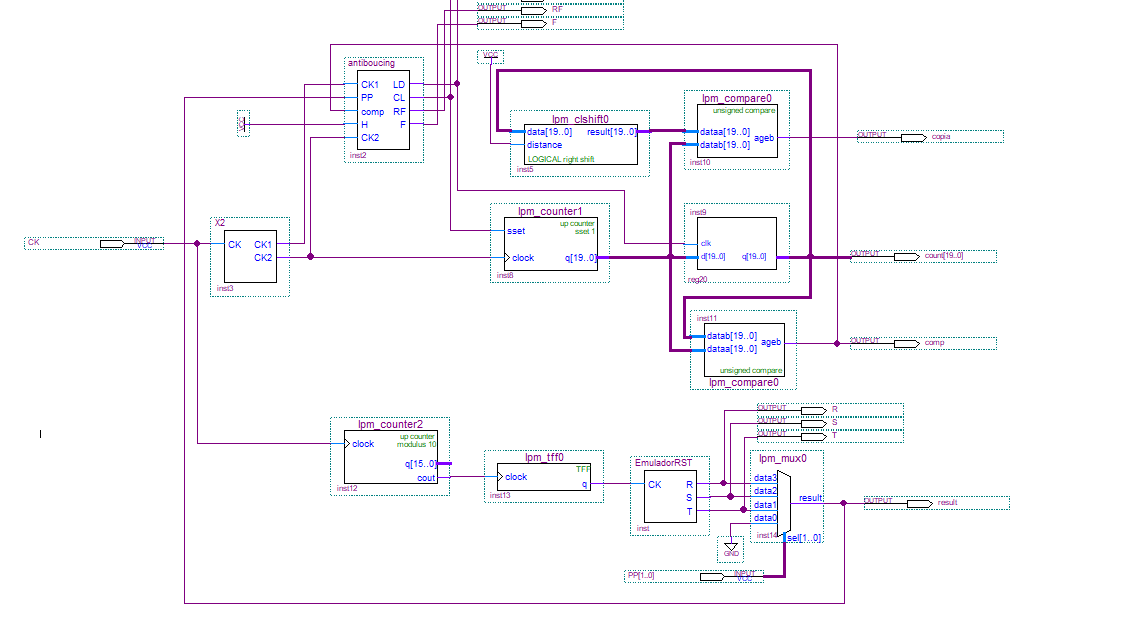
\includegraphics[width=16cm]{images/teste-antibouncing}	\label{fig:teste-antibouncing}
\end{figure}

Note que a parte inferior do circuito é idêntica ao emulador RST, a única mudança é o multiplex inserido nas saídas deste. O pino de entrada PP foi utilizado para selecionar uma das fases que seriam retroalimentadas na Unidade com o anti bouncing.

Outra mudança necessária foi a alteração do módulo do contador lpm\_counter (inst4) da Figura \ref{fig:antibouncing-uc} para 400, pois do contrário o tempo característico de bouncing seria grande demais e não seria possível ver o funcionamento do circuito.

Para a execução do teste foi inserido inicialmente o sinal R para que seja executado a cópia e depois que o sinal de referencia estivesse sincronizado, a ponta de prova foi colocada em nível baixo, e em seguida inserido o sinal S.

Utilizando o clock como 2777ns, foi gerados os resultados da Figura \ref{fig:teste-resultados-antibouncing}

\begin{figure}[!htp]
	\centering
	\caption{Simulação funcional do Gerador e Anti bouncing - Parte 1}
	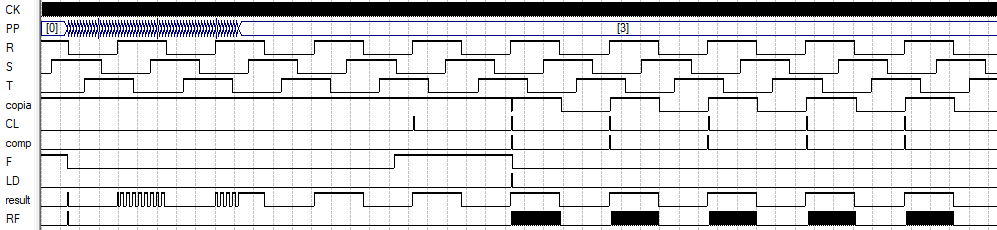
\includegraphics[width=16cm]{images/teste-resultados-antibouncing}	\label{fig:teste-resultados-antibouncing}
\end{figure}

Note que assim que começamos a criar o fenômeno de bouncing no pino PP um sinal Rf é gerado e então F fica em nível baixo até passar o tempo característico de bouncing. Quando F volta para nível alto, um pulso é dado em CL, para zerar o contador e começar a contar o valor corretamente. No final deste período é produzido novamente o CL para manter a sincronia entra a fase de referencia e um Ld para salvar o valor contado. Note que a partir deste ponto o pino cópia começa a gerar um sinal idêntico à R, e assim como o esperado vário pulsos em Rf são gerados para impedir F de ir para nível alto.

\begin{figure}[!htp]
	\centering
	\caption{Simulação funcional do Gerador e Anti bouncing - Parte 2}
	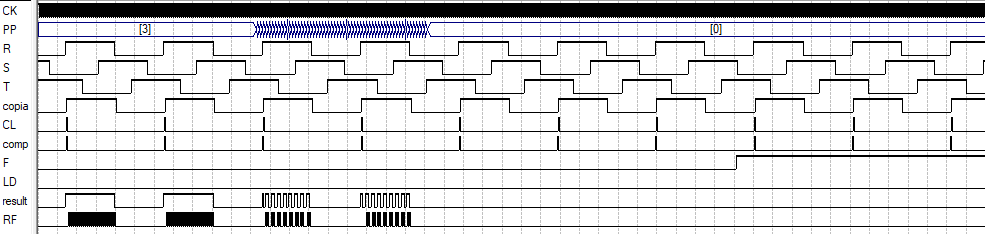
\includegraphics[width=16cm]{images/teste-resultados-antibouncing2}	\label{fig:teste-resultados-antibouncing2}
\end{figure}

Também foi simulada a retida da ponta de prova, para isto também a simulação do fenômeno de bouncing, este teste está representado na Figura \ref{fig:teste-resultados-antibouncing2}. Quando começamos a gerar a instabilidade na ponta de prova, vários Rf são feitos, até que PP se torna 0 e os pulsos em Rf para, porém, o pino cópia continua a gerar um sinal em sincronia com o sinal R.

\begin{figure}[!htp]
	\centering
	\caption{Simulação funcional do Gerador e Anti bouncing - Parte 3}
	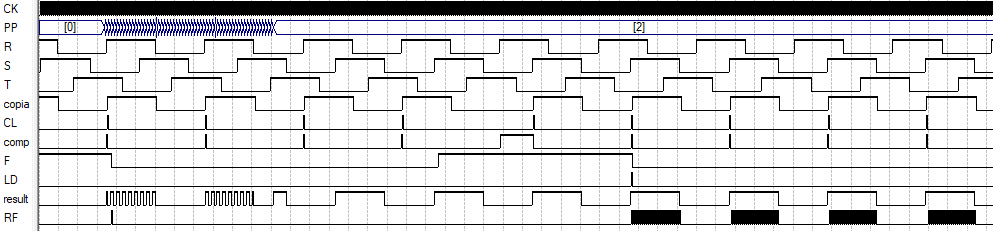
\includegraphics[width=16cm]{images/teste-resultados-antibouncing3}	\label{fig:teste-resultados-antibouncing3}
\end{figure}

Ainda neste mesmo teste, simulamos a inserção de uma nova fase de referência, representado pela Figura \ref{fig:teste-resultados-antibouncing3}. A princípio começamos a gerar a instabilidade no sinal de PP, assim como na primeira leitura, é gerado um pulso em Rf para zerar o contador da UC e começar a contar o tempo característico de bouncing. 

O fim deste tempo se dá quando F volta para o nível alto e então é gerado um sinal Cl na primeira borda de subida de S depois do tempo de bouncing. Ao fim deste período é gerado os sinais Cl e Ld, assim como na primeira leitura. Note que antes deste do primeiro Cl depois do tempo característico de bouncing o sinal de cópia ainda era igual a R, após isto, o sinal passa a ser igual ao S.

Este circuito foi testado na placa, porém não apresentou resultados positivos. Seu comportamento, quando rodando na placa, apresentava erros dos quais não fomos capazes de descobrir. Tentamos várias modificações, porém, alguns erros persistiam, outros sumiam e novos erros surgiam, impossibilitando uma conclusão precisa.

\section{Teste - Demais componentes}

Não foi possível completar e os demais componentes devido a dúvidas de implementação, testes sem sucesso e falta de tempo. Ademais, o sistema de Timeout não pôde passar por simulações de timing devido à natureza retro-alimentada do mesmo; a qual o Quartus não é capaz de processar.

\chapter{Conclusão}

Tendo em vista o projeto todo fica clara a importância da familiaridade com as ferramentas e a imporância de tê-las da melhor qualidade. O design datado do Quartus 9.0 provou-se um empecilho ao grupo, aliado à falta de visão do todo e à limitada prática com esse tipo de ferramenta e hardware.

Em retrospectiva, vários dos erros cometidos não são claros, ja que refazer o módulo defeituoso resolveu a maioria dos problemas. Contudo, foram diversas as situações que a experiência provou-se a chave.

Certamente uma abordagem incremental para o desenvolvimento teria sido saudável, implementando parte a parte e testando-as conforme o projeto avança. Contudo, este era de difícil modularização além dos segmentos já propostos, os quais eram profundamente dependentes uns dos outros.

Dos módulos propostos para o aparato, o emulador de sinais RST funcionou como proposto e foi testado na placa. Os módulo de Antibouncing foi testados em simulações de timing porém não produziu resultados positivos. Os módulos de Timeout e os leds finais não foram desenvolvidos por falta de tempo e devido aos problemas já citados.

Por fim, o projeto serve como lembrete que sob o mar de bits abstratos e caixas mágicas e objetos e vetores há um mundo complexo e duro de circuitos  e silício. Cada decisão traz uma miríade de consequências e novos desafios a serem superados. Metodologia, disciplina e atenção fazem-se imprescindíveis no mundo do software, mas imperativos no mundo do hardware.

\end{document}
